\chapter{Увеличение резкости}
\label{ch:chap3}

\definecolor{codegreen}{rgb}{0,0.6,0}
\definecolor{codegray}{rgb}{0.5,0.5,0.5}
\definecolor{codepurple}{rgb}{0.58,0,0.82}
\definecolor{backcolour}{rgb}{0.95,0.95,0.92}

\lstdefinestyle{mystyle}{
    backgroundcolor=\color{backcolour},   
    commentstyle=\color{codegreen},
    keywordstyle=\color{magenta},
    numberstyle=\tiny\color{codegray},
    stringstyle=\color{codepurple},
    basicstyle=\ttfamily\footnotesize,
    breakatwhitespace=false,         
    breaklines=true,                 
    captionpos=b,                    
    keepspaces=true,                 
    numbers=left,                    
    numbersep=5pt,                  
    showspaces=false,                
    showstringspaces=false,
    showtabs=false,                  
    tabsize=2
}
\lstset{style=mystyle}


\begin{figure}[ht]
    \centering
    
\includegraphics[width=0.5\textwidth]{house.jpg}
	\caption{Оригинал}
\end{figure}

Для того, чтобы увеличить резкость изображения, нам надо воспользоваться соответствующим ядром:
$$
    sharpen = \begin{pmatrix}
        0 & -1 & 0 \\
        -1 & 5 & -1 \\
        0 & -1 & 0 
    \end{pmatrix}
$$

\section{Через свёртку напрямую}
Делаем свёртку исходного изображения с матрицей ядра, получаем следующие результаты:

\begin{figure}[ht]
    \centering
    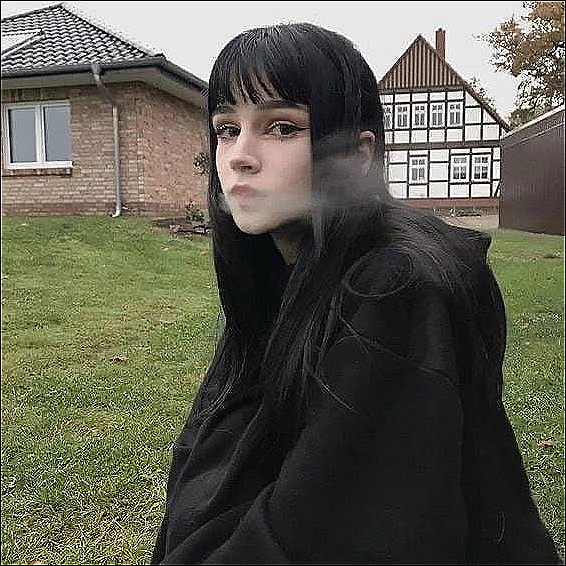
\includegraphics[width=0.6\textwidth]{house_SHARP1.png}
	\caption{Повышение резкости, применили один раз}
\end{figure}



\begin{figure}[ht]
    \centering
    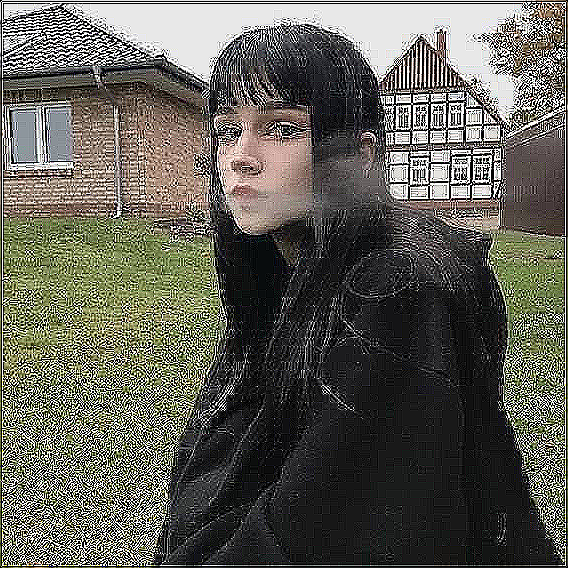
\includegraphics[width=0.6\textwidth]{house_SHARP2.png}
	\caption{Повышение резкости, применили два раза}
\end{figure}


\begin{figure}[ht]
    \centering
    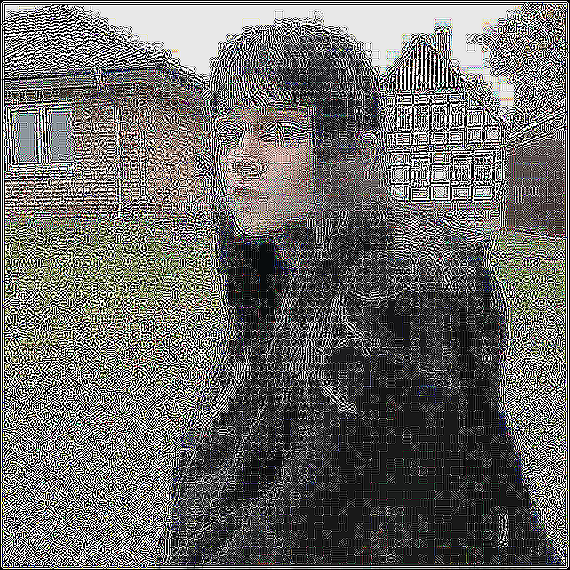
\includegraphics[width=0.6\textwidth]{house_SHARP3.png}
	\caption{Повышение резкости, применили три раза}
\end{figure}

Как можно заметить, повышение резкости позволяет нам получить края деталей или фичей изображения, и чем больше количество раз мы этом применяем, тем более выделяются основые детали.

\newpage
\section{Через использование теоремы о свёртке}
Все действия аналогичны прошлому пункту, поменялось только ядро, получим в итоге:

\begin{figure}[ht]
    \centering
    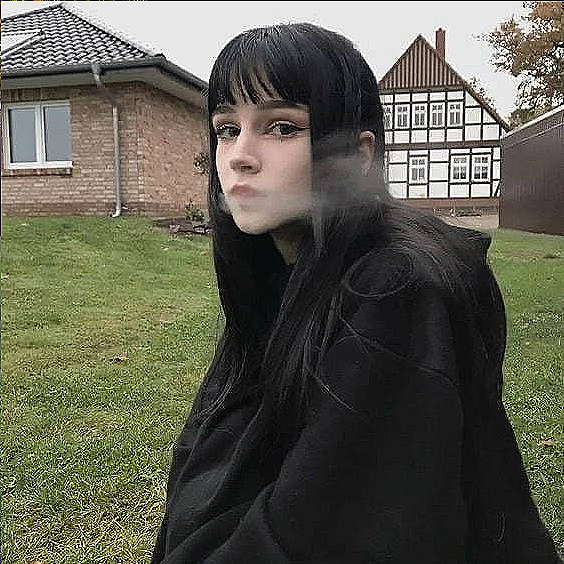
\includegraphics[width=0.6\textwidth]{house2_SHARP1.png}
	\caption{Повышение резкости, применили один раз}
\end{figure}



\begin{figure}[ht]
    \centering
    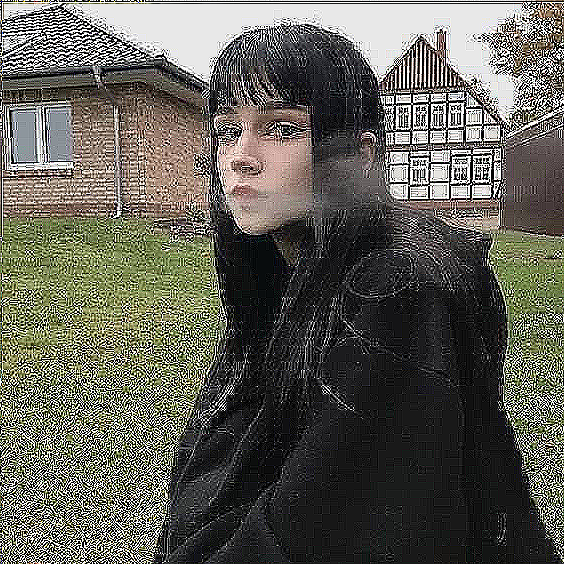
\includegraphics[width=0.6\textwidth]{house2_SHARP2.png}
	\caption{Повышение резкости, применили два раза}
\end{figure}


\begin{figure}[ht]
    \centering
    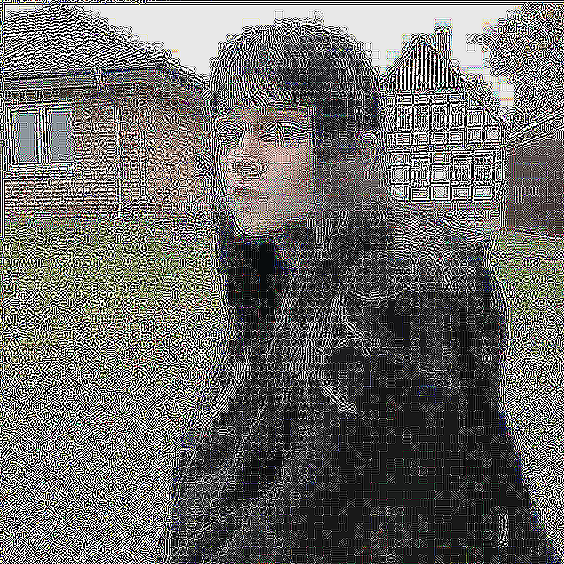
\includegraphics[width=0.6\textwidth]{house2_SHARP3.png}
	\caption{Повышение резкости, применили три раза}
\end{figure}

\section{Мини-выводы}
Замечаем снова, что теорема о свёртке работает, ведь результаты двух разных подходов совпали!

\endinput